\documentclass[11pt]{article}
\usepackage{graphicx}
\usepackage{amsmath}
\usepackage{amssymb}
\usepackage[top=0.75in, bottom=1.25in, left=1in, right=1in,includefoot]
{geometry}
\usepackage{fancyhdr}
\usepackage{mathpartir}
\usepackage{appendix}
\usepackage[backend=biber,style=numeric,sorting=none]{biblatex} % bibliography, install biber otherwise it will not work
\addbibresource{2_De_Paiva.bib}
\usepackage[colorlinks=true, linkcolor=cyan, citecolor=cyan, urlcolor=blue]{hyperref}
\usepackage{blindtext}
%remove the line above

\DefineBibliographyStrings{english}{
    % add bibliography page to table of contents
    bibliography = {References},
}

\pagestyle{fancy}
\fancyhead[L]{\fancyhdrbox[c]{\Large \slshape \sffamily 
Lambda-Calculi for Logics}}
\fancyhead[C]{}
\fancyhead[R]{\large \sffamily \bfseries Valeria De Paiva }

\fancyfoot[L]{\fancyhdrbox[b]{\sffamily \small Compiled By: \\ 
\normalsize \sffamily Adam Brohl, Ellen Whalen, Vincent Chan}}
%Change the names above to your names

\fancyfoot[C]{\thepage}
\fancyfoot[R]{\fancyhdrbox[b]{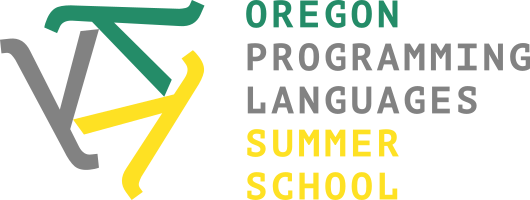
\includegraphics[height=0.35in]{oplssLogo.png}}}
\renewcommand{\footrulewidth}{0.5pt}

\setlength{\parindent}{0pt}
\setlength{\parskip}{2ex}
\setlength{\headheight}{1.25in}

\begin{document}
\thispagestyle{plain}
\begin{center}
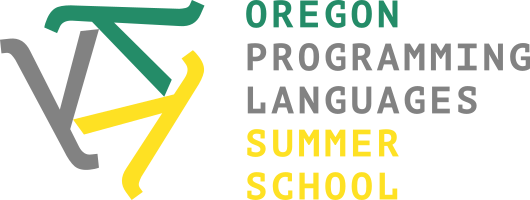
\includegraphics[width=3in]{oplssLogo.png}\\[2\parskip]
\sffamily \LARGE \slshape Lambda-Calculi for Logics
--- \upshape Valeria De Paiva \\[2ex]
\href{https://github.com/vcvpaiva/DialecticaCategories/blob/master/OPLSS2025/OregonLecture2.pdf}{\large Lecture 2 - \slshape June 24, 2025}
\end{center}


\section{Classical Modal Logic}

\begin{itemize}
    \item Modal logic is the most successful logical framework in CS
    \item $\square A = A$ is necessarily the case, A holds all of the time/at every world, etc.
    \item $\Diamond A = A$ is possibly the case, A holds at some time/some world, etc.
    \item Temporal logic, knowledge operators, BDI models, denotational semantics, effects, security modeling and verification, databases, etc. built off of classical modal logic - until about 20 years ago, it was the main modality considered
\end{itemize}

\section{Constructive Reasoning}

\begin{itemize}
    \item If I ask you `is there an $x$ such that $P(x)$'?, I'm happier with the constructive reasoning answer `yes, $x_0$' than with the classical reasoning answer `yes, for all $x$ it is not the case that not $P(x)$' (in other words, specialization rather than $\neg \forall  x. (\neg P(x))$)
    \item Why: want reasoning to be as precise and safe as possible. To do this, use constructive reasoning as much as possible, classical if need be, but tell me where (classical can give a good indication for which direction to go for)
    \item Today is more about constructive modality
\end{itemize}

\section{Intuitionistic Modal Logic}

Basic idea: Modalities over intuitionistic propositional basis: \[\land, \lor, \implies, \lnot\]
Start here, then build. We want to put constructive modalities on top of constructive bases. Some questions arise:

\begin{itemize}
    \item How do we choose the best constructive modalities? Certain properties of certain logics work better with certain systems.
    \item Which intuitionistic basis should we choose?
    \item How do modalities/systems relate to each other?
    \item Why are there so many modal logics?
    \item Which theorems should we work hard to preserve?
    \item Which are the most useful applications?
\end{itemize}

Simpson's 1994 PhD thesis is a good place for an overview of intuitionistic modal logic\cite{Simpson1994ThePT}.

\section{Constructive Modal Logic}
Constructive logic is a logical basis for programming via Curry-Howard correspondences. 
A lot of places use `constructive logic' and `intuitionistic logic' interchangeably, but constructive logic is a broader term that includes intuitionistic logic and other logics.
While intuitionistic logic determines the truth of a proposition by the existence of a proof, constructive logic focuses on the existence of a witness for a proposition\cite{Pfenning2017ConstructiveLogic}.
Modalities are useful in computing, so constructive modalities ought to be twice as useful. But which constructive modalities should we use? Have we ``gotten to the right one'' yet?
\begin{itemize}
    \item Usual pheonmenon: classical facts can be 'constructivized' in many different ways depending on expected behavior and desired tools. Hence constructive notions multiply which leads to too many choices. Our goal is to extract the best system we can.
    \item Operators $\square$ and $\Diamond$ (like $\forall$/$\exists$) are not interdefinable, but they shouldn't be \textit{completely} separate since they are related.
    \item The proof theory of modal logic is difficult, so we sometimes don't end up with the logics we expect/want.
    \item In finding good systems of constructive modal logic, lots of extra syntax/semantics have been added: hypersequents, labelled deduction systems, (linear) nested sequents, tree-sequents...
\end{itemize}

\section{Intuitionistic Modal Logic and Applications (IMLA)}
IMLA is a loose association bringing together researchers in the fields of philosophy, math, logic, and computer science in the hopes that they would be able to share their perspectives and benefit from others' research on intuitionistic modal logics and modal type theories. This has been semi-successful, but in the end, the researchers' different backgrounds leads people to often talk past one another. 

IMLA had some early successes using CS4 and Lax logics, but due to the reasons detailed in the rest of these notes, some of the gains in modal type theories ended up not working out as well as expected.

\section{Constructive S4 (CS4)}

\begin{itemize}
    \item Better behaved modal system, used by Gödel and Girard
    \item Goal: think linearly in certain cases and classically in others.
    \item Usual intuitionistic axioms plus MP, Nec rules and:
\end{itemize}

% below this point I haven't made a ton of edits because I ended up getting kind of lost during the lecture. A fair bit of this seems to be taken directly from the slides, and probably should be reworded -Ellen 

\textbf{Modal Axioms}\cite{balbiani2024constructives4modallogics}\cite{Natasha2001CategoricalKripkeCS4}

\begin{itemize}
    \item $\square(A \rightarrow B) \rightarrow (\square A \rightarrow \square B)$
    \item $\square A \rightarrow A$
    \item $\square A \rightarrow \square\square A$
    \item $\square(A \rightarrow \Diamond B) \rightarrow (\Diamond A \rightarrow \Diamond B)$
    \item $A \rightarrow \Diamond A$ (If something is true than it is possibly true)
\end{itemize}

\section{CS4 Sequent Calculus}
S4 modal sequent rules first discussed in 1957 by Ohnishi and Matsumoto:

$$\frac{\Gamma, A \vdash B}{\Gamma, \square A \vdash B}$$
$$\frac{\square\Gamma \vdash A}{\square\Gamma\vdash\square A}$$
$$\frac{\square\Gamma, A \vdash B}{\square\Gamma,\Diamond A \vdash B}$$
$$\frac{\Gamma\vdash A}{\Gamma \vdash \Diamond A}$$

Cut-elimination works, for classical and intuitionistic basis.

\section{CS4 Natural Deduction}
Natural Deduction (ND) has a more complicated rule

$$\frac{\square\Gamma\vdash A}{\square\Gamma\vdash\square A}$$

Abramsky's computational interpretation of linear logic leads to calculus that does not satisfy substitution\cite{abramsky1993_linear_logic}.

Given proofs:
\begin{mathpar}
    \infer{\infer{\Box A_1 \\ \Box A_2}{B}}{\Box B}\and
    \infer{C \to \Box A_1 \\ C}{\Box A_1}
\end{mathpar}

We cannot derive $\Box B$ from $C \to \Box A_1, \Box A_2$ and $C$ by combining the two proofs because $\Box B$ requires $\Box C$ in the context, which is not the case for the second proof.

One solution builds the substitutions into the rule as:

$$\frac{\Gamma \vdash \square A_1,...,\Gamma\vdash\square A_k\space \square A_1,...,\square A_k \vdash B}{\Gamma\vdash\square B}(\square I)$$

Another solution: Prawitz uses a notion of "essentially modal subformula" to guarantee substituitivity in his monograph and makes several improvements. Overall, CS4 is ``very well behaved'' but still has issues.


\section{CS4: Properties/Theorems}
\begin{itemize}
    \item Axioms satisfy deduction theorem, are equivalent to sequents,
    \item Sequents satisfy cut-elimination, sub-formula propery
    \item ND is equivalent to sequents
    \item ND satisfies normalization, ND assigns $\lambda$-terms curry howard equivalent
    \item Categorical model: monoidal comonad plus box-strong monad
\end{itemize}

Issues:
\begin{itemize}
    \item Idempotency of comonad ($\square A = \square \square A$) is not warranted and causes problems. Ideally, proofs should not be isomorphic - proving both directions is OK, but keeping them separate is much better.
    \item Rules are impure: in a couple of cases, to introduce $\square$ on the right, you need to already know it on the left.
\end{itemize}

\section{Dual Intuitionistic and Modal Logic}
\begin{itemize}
    \item Following LL can define a dual system for $\square$-only modal logic
    \item Less impurity on rules, less commuting conversions, but what about $\Diamond$? what about other modal systems?
\end{itemize}

\section{Lax Logic}

Using Curry-Howard ``backwards'' to get the logic by dropping the terms

\textbf{Motivation}: Moggi's computational lambda calculus, an intuitionistic modal metalanguage for denotational semantics for programming language features: non-termination, differing evaluation strategies, non-determinism, side-effects are examples

\subsection{Lax Modality Axioms}

$A \rightarrow \Diamond A$
$\Diamond\Diamond A \rightarrow \Diamond A$
$(A \rightarrow B) \rightarrow (\Diamond A \rightarrow \Diamond B)$

\section{System Lax}

Also called CL-logic (for computational lambda calculus)

\subsection{Lax Logic Properties}

\begin{itemize}
    \item Axioms, sequents, and ND are equivalent 
    \item Deduction theorem holds, as does substitution and subject reduction
    \item The term calculus associated is strongly normalizing
    \item The reduction system given is confluent 
    \item Cut elimination holds
    \item Lax logic (PLL) categorical mods as expected
\end{itemize}


\section{Constructive K}
Although Lax Logic and CS4 both have all important properties hold, modalities built on top of them are more difficult. We want properties like $\Diamond(A\lor B) \cong \Diamond A \lor \Diamond B$ and $\Diamond \bot \cong \bot$ (derivable from one another) which CS4 doesn't allow.

\begin{itemize}
    \item Constructive K comes from proof-theoretical intuitions provided by Natural Deduction formulations of logic
    \item Note: only one rule for each connective, also $\Diamond$ depends on $\square$
\end{itemize}

\subsection{Properties}

\begin{itemize}
    \item Dual-context only for Box fragment
    \item For box-fragment OK. Have subject reduction, normalization and confluence for associated lambda-calculus
    \item Have categorical models, but too constrainted?
    \item Kripe semantics OK
\end{itemize}
Constructive K ends up having a ``disturbing'' non-uniformity of systems, so more work is necessary.

\section{Alternatives}
Many alternatives exist, but the main one that is used is described by Simpson \cite{Simpson1994ThePT}
\begin{itemize}
    \item Simpson 1994 PhD: robust system for geometric ND theories for intuitionistic modal logic
    \item Justified by translation into intuitionistic first-order, recovers many of the systems in the literature
    \item Strong normalization and confluence proved for all the systems
    \item Normalization establishes completeness of cut-free sequent calculi and decidability of some of the systems
    \item decidable systems satisfy "finite model property"
\end{itemize}
The main problem with Simpson and the other alternatives is the lack of categorical models.

\section{Wanted}

\begin{itemize}
    \item Constructive modal logics with axioms, sequents and natural deduction formulations, proved equivalent
    \item Cut-elimination, finite model property, (strong) normalization, confluence, and decidability
    \item Algebraic, Kripke, and categorical semantics
    \item Translating proofs more than simply theorems
    \item A broad view of constructive and/or modality
    \item If possibile, limitative results
\end{itemize}

\section{Avron's Desiderata}

\begin{itemize}
    \item Should be able to handle a great diversity of logics, especially the traditional ones
    \item Should be independent of any particular semantics
    \item Structures should not be too complicated, yield a "real" subformula property
    \item Rules of inference should have a small fixed number of premises, and a local nature of application
    \item Should give us a better understanding of the logics and the differences between them
\end{itemize}

\section{Diamond over Disjunction}

Distribution of possibility over disjunction binary and nullary: Holds in IS4 (Simpson), but not in CS4

$$\Diamond(A \lor B) \rightarrow \Diamond A \lor \Diamond B$$
$$\Diamond\bot \rightarrow \bot$$

\begin{itemize}
    \item Distribution is canonical for classical modal logics, but many constructive modal logics don't satisfy it.
    \item Consequence: adding excluded middle gives you back classical modal logic
\end{itemize}

\section{Labelled vs Unlabelled}

\begin{itemize}
    \item Introduction rule for $\square$ says if A holds at every world y visible from x then $\square A$ holds at x.
    \item Simpson two kinds of hypotheses:  x : A means that the modal formula A is true in the world x; xRy, which says that world y is accessible from world x
    \item How reasonable is it to have your proposed semantics as part of your syntax?
    \item Proof-theoretic properties achieved, but no categorical semantics
\end{itemize}

\newpage
\printbibliography[heading=bibintoc]
\end{document}
